\documentclass{standalone}
\usepackage{tikz}
\usepackage{ctex,siunitx}
\usepackage{tkz-euclide}
\usepackage{amsmath}
\usetikzlibrary{patterns, calc}
\usetikzlibrary {decorations.pathmorphing, decorations.pathreplacing, decorations.shapes,}
\begin{document}
\small
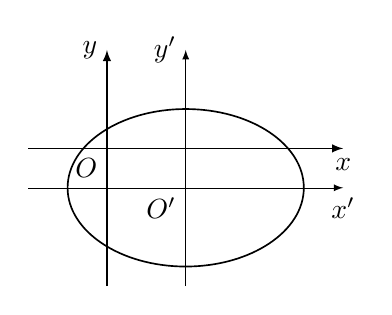
\begin{tikzpicture}[>=latex,scale=0.5]
  \draw[thin,->](-2,0)--(6,0)node[below]{$x$};
  \draw[thin,->](0,-3.5)--(0,2.5)node[left]{$y$};
  \draw[very thin,->](-2,-1)--(6,-1)node[below]{$x'$};
  \draw[very thin,->](2,-3.5)--(2,2.5)node[left]{$y'$};
  \tkzDefPoints{0/0/O,3/-4/A,2/-1/O',5/2/B,3/-2/C}
  \draw[semithick](2,-1)ellipse(3 and 2);
  \tkzLabelPoints[below left](O,O')
\end{tikzpicture}
\end{document}